\documentclass{neu_handout}
\usepackage{url}
\usepackage{amssymb}
\usepackage{amsmath}
\usepackage{marvosym}
\usepackage{graphicx}
\graphicspath{ {images/} }
\everymath{\displaystyle}

% Professor/Course information
\title{Update 1}
\author{Emily Dutile, Vyshaal Narayanam, Xiwen Song, Yu Tian}
\date{November 2017}
\course{CS6220}{Data Mining Techniques}

\begin{document}

\section*{1. Exploratory analysis}
With the Yelp Open Dataset\footnote{\url{https://www.yelp.com/dataset}} consisting of 4.7 million reviews, 156,000 business, and 12 metropolitan areas, we needed to filter out a signification amount of data and perform some further exploration in order to set potential thresholds to either include or exclude particular data. Below is the Yelp Dataset schema.

\begin{center}
Yelp Data Schema\\
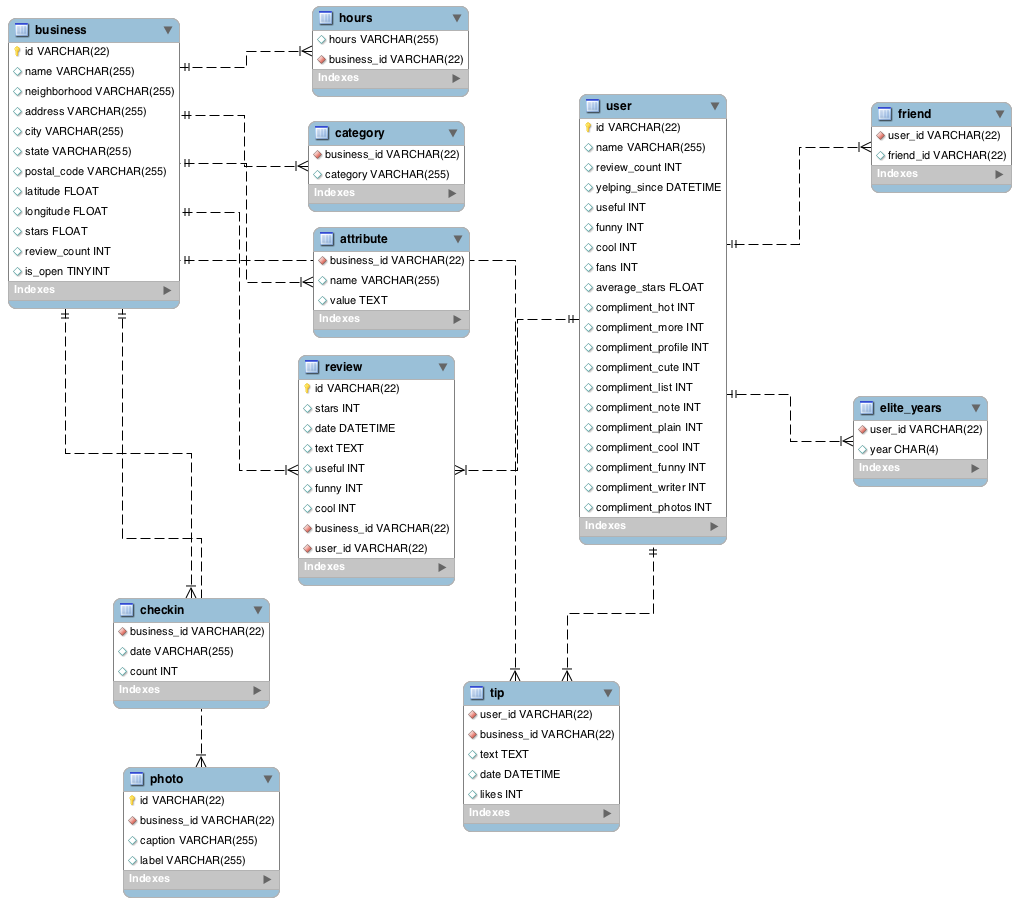
\includegraphics[width=150mm,scale=0.5]{schema}\\
\end{center}

In order to answer our original questions, we had to narrow down and verify what attributes we needed from our data set.\\

The following tables are used to answer question 1:\\

\begin{center}
Business\\
\begin{tabular}{|l|l|}
\hline
id  \\ \hline
name  \\ \hline
neighborhood  \\ \hline
city  \\ \hline
longitude  \\ \hline
latitude  \\ \hline
stars  \\ \hline
\end{tabular}
\end{center}

\begin{center}
Review\\
\begin{tabular}{|l|l|}
\hline
business\_id  \\ \hline
user\_id  \\ \hline
stars  \\ \hline
date  \\ \hline
text  \\ \hline
funny  \\ \hline
useful  \\ \hline
\end{tabular}
\end{center}

\begin{center}
Tip\\
\begin{tabular}{|l|l|}
\hline
business\_id  \\ \hline
text  \\ \hline
likes  \\ \hline
\end{tabular}
\end{center}

The following tables are used to answer question two:

\begin{center}
Business\\
\begin{tabular}{|l|l|}
\hline
id  \\ \hline
name  \\ \hline
neighborhood  \\ \hline
city  \\ \hline
longitude  \\ \hline
latitude  \\ \hline
stars  \\ \hline
\end{tabular}
\end{center}

\begin{center}
Category\\
\begin{tabular}{|l|l|}
\hline
business\_id  \\ \hline
category  \\ \hline
\end{tabular}
\end{center}


To get started, we created local databases and imported the given SQL file using MySQL Server and PyCharm in our development environment. Using Jupyter Notebooks, we have created some basic visualizations and calculations in order to better filter and preprocess our data.

\section*{2. Extraction Update}
Our original questions: \\
(1) What topics are discovered frequently in reviews and do they correlate to a positive or negative review? What should a restaurant focus on to make their rating/reviews better? \\
(2) What neighborhoods in Pittsburgh have the best cuisine selection? \\

Number of Pittsburgh neighborhoods: \\
Number of categories/cuisines: \\
Categories/cuisines: \\

In order to tell authentic from trendy, we have joined the business, category and attributes table.\\


We have picked restaurants with more than 200 reviews:


\end{document}
